% TU Delft beamer template
% Author: Erwin Walraven (initial version was created by Maarten Abbink)
% Delft Universiy of Technology

\documentclass{beamer}
\usepackage[english]{babel}
\usepackage{calc}
\usepackage[absolute,overlay]{textpos}
\usepackage{graphicx}
\usepackage{subfig}
\usepackage{amsmath}
\usepackage{amsfonts}
\usepackage{amsthm}
\usepackage{mathtools}
\usepackage{comment}
\usepackage{MnSymbol,wasysym}
\usepackage{import}
\usepackage{standalone}
\usepackage{tikz}

\newcommand{\circumeq}{\mathrel{\widehat{=}}}
\setbeamertemplate{navigation symbols}{} % remove navigation symbols
\mode<presentation>{\usetheme{tud}}

% BIB SETTINGS
\usepackage[backend=bibtex,firstinits=true,maxnames=30,maxcitenames=20,url=false,style=authoryear]{biblatex}
\bibliography{bibfile}
\setlength\bibitemsep{0.3cm} % space between entries in the reference list
\renewcommand{\bibfont}{\normalfont\scriptsize}
\setbeamerfont{footnote}{size=\tiny}
\renewcommand{\cite}[1]{\footnote<.->[frame]{\fullcite{#1}}}

\title[]{Connecting the "Dots": \\
Topology Optimization for Fiber-Reinforced Composites}
\institute[]{University of Bologna, Italy \\ Delft University of Technology, The Netherlands}
\author{Y. Gandhi \and G. Minak \and A.M. Arag{\'o}n}
%\date{}

\begin{document}
{
\setbeamertemplate{footline}{\usebeamertemplate*{minimal footline}}
\frame{\titlepage}
}

{\setbeamertemplate{footline}{\usebeamertemplate*{minimal footline}}

}

\begin{frame}{Simultaneous Fiber \& Composite \\ Topology Optimization}
    \begin{figure}[!ht]
        \centering
        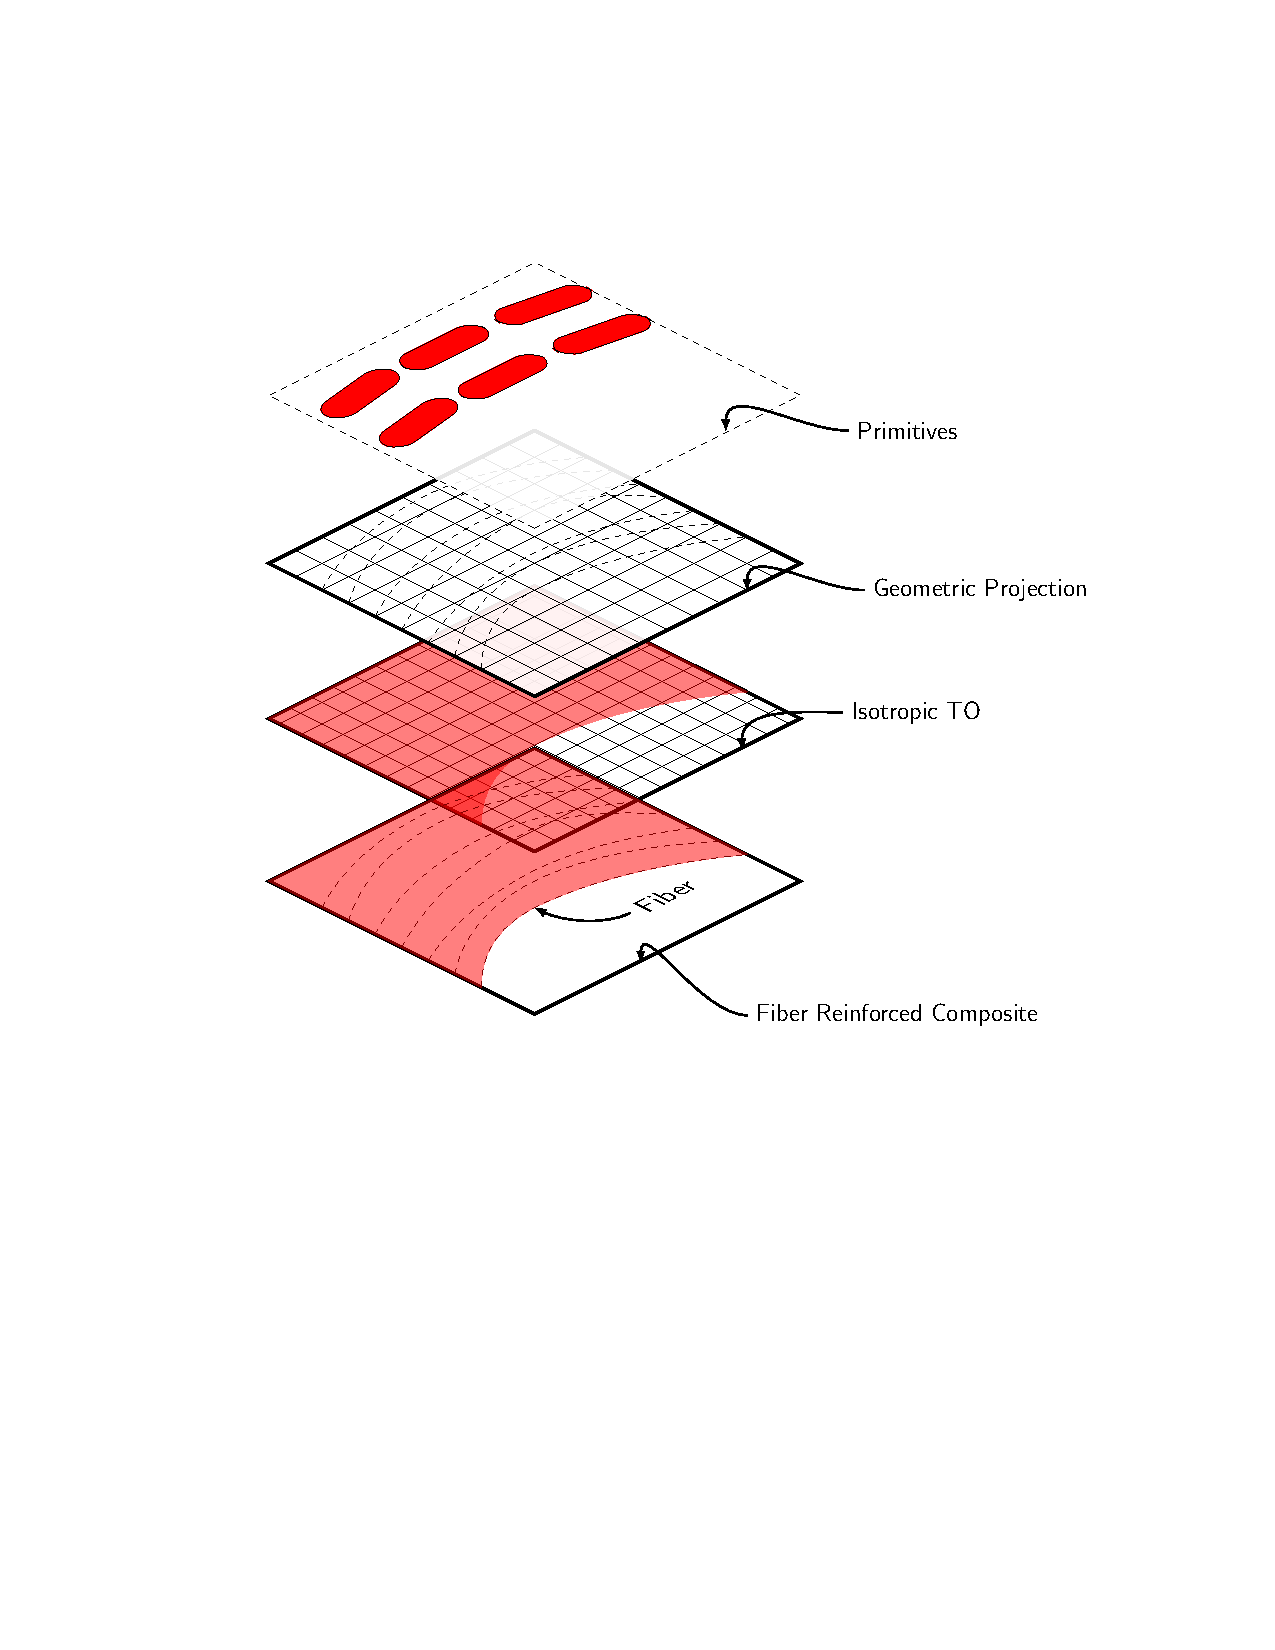
\includegraphics[width=0.8\textwidth]{./Schematics/GTO_FRC.pdf}
        \label{fig:GTO_FRC}
    \end{figure}
\end{frame}

\begin{frame}{Topological }
    Computing Topological sensitivity field to locate optimal fiber
    \begin{equation*}
        \psi(\Omega)=\frac{1}{2}\int_{\Omega}\sigma(\mathbf{u})
        \cdot\varepsilon(\mathbf{u})
    \end{equation*}
    \begin{equation*}
        TD(\hat{x}) = \underset{\epsilon\rightarrow 0}{\text{lim}}
        \frac{\psi_{\epsilon}(\Omega)-\psi(\Omega)}{f(\epsilon )}
    \end{equation*}
\end{frame}

\begin{frame}{Algorithm}
    \begin{figure}[!ht]
        \centering
        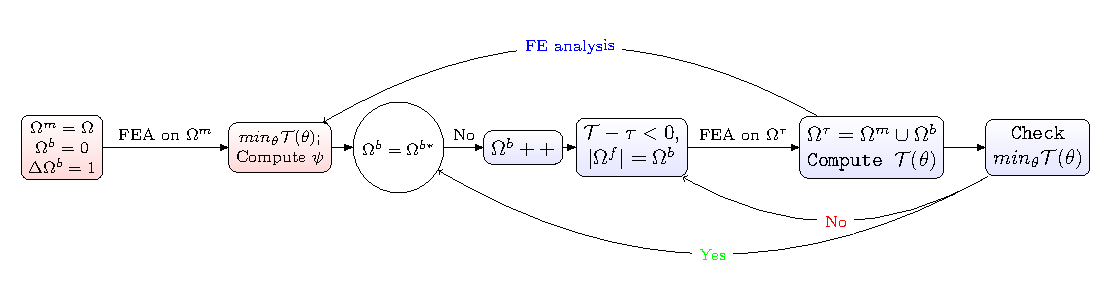
\includegraphics[width=1\textwidth]{./Schematics/treenodes.pdf}
        \label{fig:treenode}
    \end{figure}
    \begin{enumerate}
        \item Initilaized $\Omega^{m}=\Omega$
        \item $\Omega^{b}++ \Rightarrow \rho_{be}$;
              Compute $\mathcal{T}(\theta)\circumeq \psi$
        \item Check desired fiber fraction
              \begin{enumerate}
                  \item $\Omega^{b}++ \Rightarrow \rho_{be}$
              \end{enumerate}
    \end{enumerate}
\end{frame}

\end{document}
